% Original work copyright 2014 Jean-Philippe Eisenbarth
% Modified work copyright 2016 of Brendan Duke and Jordan Viveiros.

% This program is free software: you can
% redistribute it and/or modify it under the terms of the GNU General Public
% License as published by the Free Software Foundation, either version 3 of the
% License, or (at your option) any later version.
% This program is distributed in the hope that it will be useful,but WITHOUT ANY
% WARRANTY; without even the implied warranty of MERCHANTABILITY or FITNESS FOR A
% PARTICULAR PURPOSE. See the GNU General Public License for more details.
% You should have received a copy of the GNU General Public License along with
% this program.  If not, see <http://www.gnu.org/licenses/>.
%added comment
% Based on the code of Yiannis Lazarides
% http://tex.stackexchange.com/questions/42602/software-requirements-specification-with-latex
% http://tex.stackexchange.com/users/963/yiannis-lazarides
% Also based on the template of Karl E. Wiegers
% http://www.se.rit.edu/~emad/teaching/slides/srs_template_sep14.pdf
% http://karlwiegers.com
\documentclass{scrreprt}
\usepackage{listings}
\usepackage{underscore}
\usepackage[bookmarks=true]{hyperref}
\usepackage[utf8]{inputenc}
\usepackage[english]{babel}
\usepackage{xcolor}
\usepackage{indentfirst}
\usepackage[section]{placeins}
\usepackage{graphicx}
\usepackage{graphics}
\usepackage{longtable}
\usepackage{booktabs}
\providecommand{\tightlist}{%
  \setlength{\itemsep}{0pt}\setlength{\parskip}{0pt}}
\hypersetup{
    bookmarks=false,    % show bookmarks bar?
    pdftitle={Text to Motion User Manual},    % title
    pdfauthor={David Pitkanen, et al.},                     % author
    pdfsubject={TeX and LaTeX},                        % subject of the document
    pdfkeywords={TeX, LaTeX, graphics, images}, % list of keywords
    colorlinks=true,       % false: boxed links; true: colored links
    linkcolor=blue,       % color of internal links
    citecolor=black,       % color of links to bibliography
    filecolor=black,        % color of file links
    urlcolor=purple,        % color of external links
    linktoc=page            % only page is linked
}%
\def\myversion{0.0}
\date{}
%\title
\usepackage{hyperref}
\begin{document}

\begin{flushright}
    \rule{16cm}{5pt}\vskip1cm
    \begin{bfseries}
        \Huge{User Manual }\\
        \vspace{1.4cm}
        for\\
        \vspace{1.4cm}
        CS 4ZP6 Capstone Project\\
        \vspace{1.4cm}
        \LARGE{Version \myversion}\\
        \vspace{1.4cm}
        Prepared by Brendan Duke, Andrew Kohnen, Udip Patel, David Pitkanen, Jordan Viveiros\\
        \vspace{1.4cm}
        McMaster Text to Motion Database\\
        \vspace{1.4cm}
        \today\\
    \end{bfseries}
\end{flushright}

\listoffigures


\tableofcontents

\chapter*{Revision History}

\begin{center}
    \begin{tabular}{|c|c|c|c|}
        \hline
            Name & Date & Reason For Changes & Version\\
        \hline
	    David Pitkanen & September. 25th, 2015 & Initial Version & 0.0\\
        \hline
    \end{tabular}
\end{center}

\section{Legal and Copyright Information}

This program, Text-To-Motion is free software: and you can redistribute it
and/or modify it under the terms of the GNU General Public License as published
by the Free Software Foundation, either version 3 of the License, or (at your
option) any later version.

This program is distributed in the hope that it will be useful, but WITHOUT ANY
WARRANTY; without even the implied warranty of MERCHANTABILITY or FITNESS FOR A
PARTICULAR PURPOSE.  See the GNU General Public License for more details.

You should have received a copy of the GNU General Public License along with
this program.  If not, see http://www.gnu.org/licenses/.


\section{Introduction}

The Text-to-Motion software suite consists of a web application, an HTTP
TensorFlow server, and human pose estimator model training code. These
components can either be used together with a unified web interface, or
individually using their respective programming interfaces.

The web application can be used to extract a low dimensional representation of
the human body dynamics present in a video or the static pose of a person that
has been captured in a picture.

This web application will allow a user to upload a video or an image that
contains at least one person in it. If the user uploaded an image, a static
description of the human pose will be extracted from the image and stored in a
database. If the user uploads a video a representation of the human motion
present in that video will be stored on the same database.  The motion or pose
that the application extracts from the video or image can be displayed by the
application.

The motion or pose that is captured by the application is represented by 16
(x,y) coordinates that reference the point pixels where 16 key body parts are
located in the frame or picture of interest.  The way these 16 coordinates
change from frame to frame can be used to model human motion.  These points
represent the positions of the head, shoulders, knees, wrists, elbows, hips,
and feet (a total of 16 points) of the person on the 2D picture/video.

In addition the application offers a search function.  If the media that is
inputted includes a description of the motion or pose then other users may
query the database.  The database will perform a search for keywords and return
motions or poses that match the keywords.

In order to do inference to find human joint positions, the web application
server queries a standalone backend server, the ``TensorFlow HTTP Server''.
This server is solely responsible for handling requests to do human pose
inference, which it accepts via HTTP POST requests containing a URL indicating
the media (image or video) at should be pose-estimated. The TensorFlow HTTP
Server then returns an HTTP response containing the joint positions.

The human pose estimator model training code is a module containing
self-contained set of TensorFlow code that is able to train a state-of-the-art
human pose estimator for single-person images on the MPII Human Pose dataset
(\url{http://human-pose.mpi-inf.mpg.de/}). This code is much in the style of
the TensorFlow Slim image classification code
(\url{https://github.com/tensorflow/models/tree/master/inception/inception}),
which uses the ImageNet dataset, and could be re-used by researchers working on
human pose estimation in the computer vision community.

\section{Purpose}

The initial purpose for developing this tool was to generate a data source that
would be useful to machine learning researchers and developers.  Machine
learning researchers are interested in creating models from labelled data.  A
tool that can find the joint positions in images and videos is obviously a good
method to generate data that is labelled with joint positions.

There are many large data sources (videos and images) that have been annotated
with natural language describing their human motion. This motion/joint positions
extracting tool could be used to enrich data sources annotated with natural
language.  These data sources would contain related natural language  and
motion descriptions and so would be good sources that create connections
between these different domains.

However this project can be used as a tool for other applications as well, since
the task of finding the human motion in a video or pose in a picture is useful
in its own right.

Since it can keep track of human body positions on a screen it can also be used
potentially for training people how to move or as an aid in games where motion
needs to be kept tack of.

\subsection{Objective of User Manual}

This document has been written for people wishing to use the Text-To-Motion web
application and software suite.  The document describes how to get the
application to perform its basic functions, such as display videos that have
been captioned with joint positions and how to search the database for
pre-captioned motions and poses.

This manual also provides technical guidance such as installation instructions
and troubleshooting advice.

\subsubsection{Background Applications}

Many applications on the market right now implement similar functionality to
our Text-to-Motion program.  We can take PlayStation's Move Motion Controller
and the Wii Motion plus as examples.  Both of these products allow users to
play video games by using motion instead of a controller.  In addition motion
analysis is common to help improve athletes and help to prevent injury also
helps in rehab because calculate forces imposed due to movements commonly
studied at universities and there is even an app on the iTunes store called the
Sports Motion Analyzer.

\section{Roadmap}

This text-to-motion software will have two broad classes of potential users.
The first class will wish to use the web application as it is available on our
website.  These users will simply navigate to the site using a browser and take
advantage of the framework provided. However the second class will wish to take
the software we provide on GitHub and host this software as their own website
to collect their own data and provide their own services.

Both of these types of users will have their own challenges.  Of course users
who wish to become hosts will themselves have users of their own so the first
class of potential users' problems will be of interest to the second class.

We therefore break this section down into two streams.  The first stream shows
the challenges that are of interest to users of the web application once it has
been installed.  The second stream is for problems that will only be of
interest to potential users who wish to get the software running on their own
server.

\subsection{Roadmap: Web clients}

The web application we provide will have many pages that have different
functionalities.  The navigational structure of the application is shown in
Figure \ref{fig:navStruct}.

\begin{figure}
  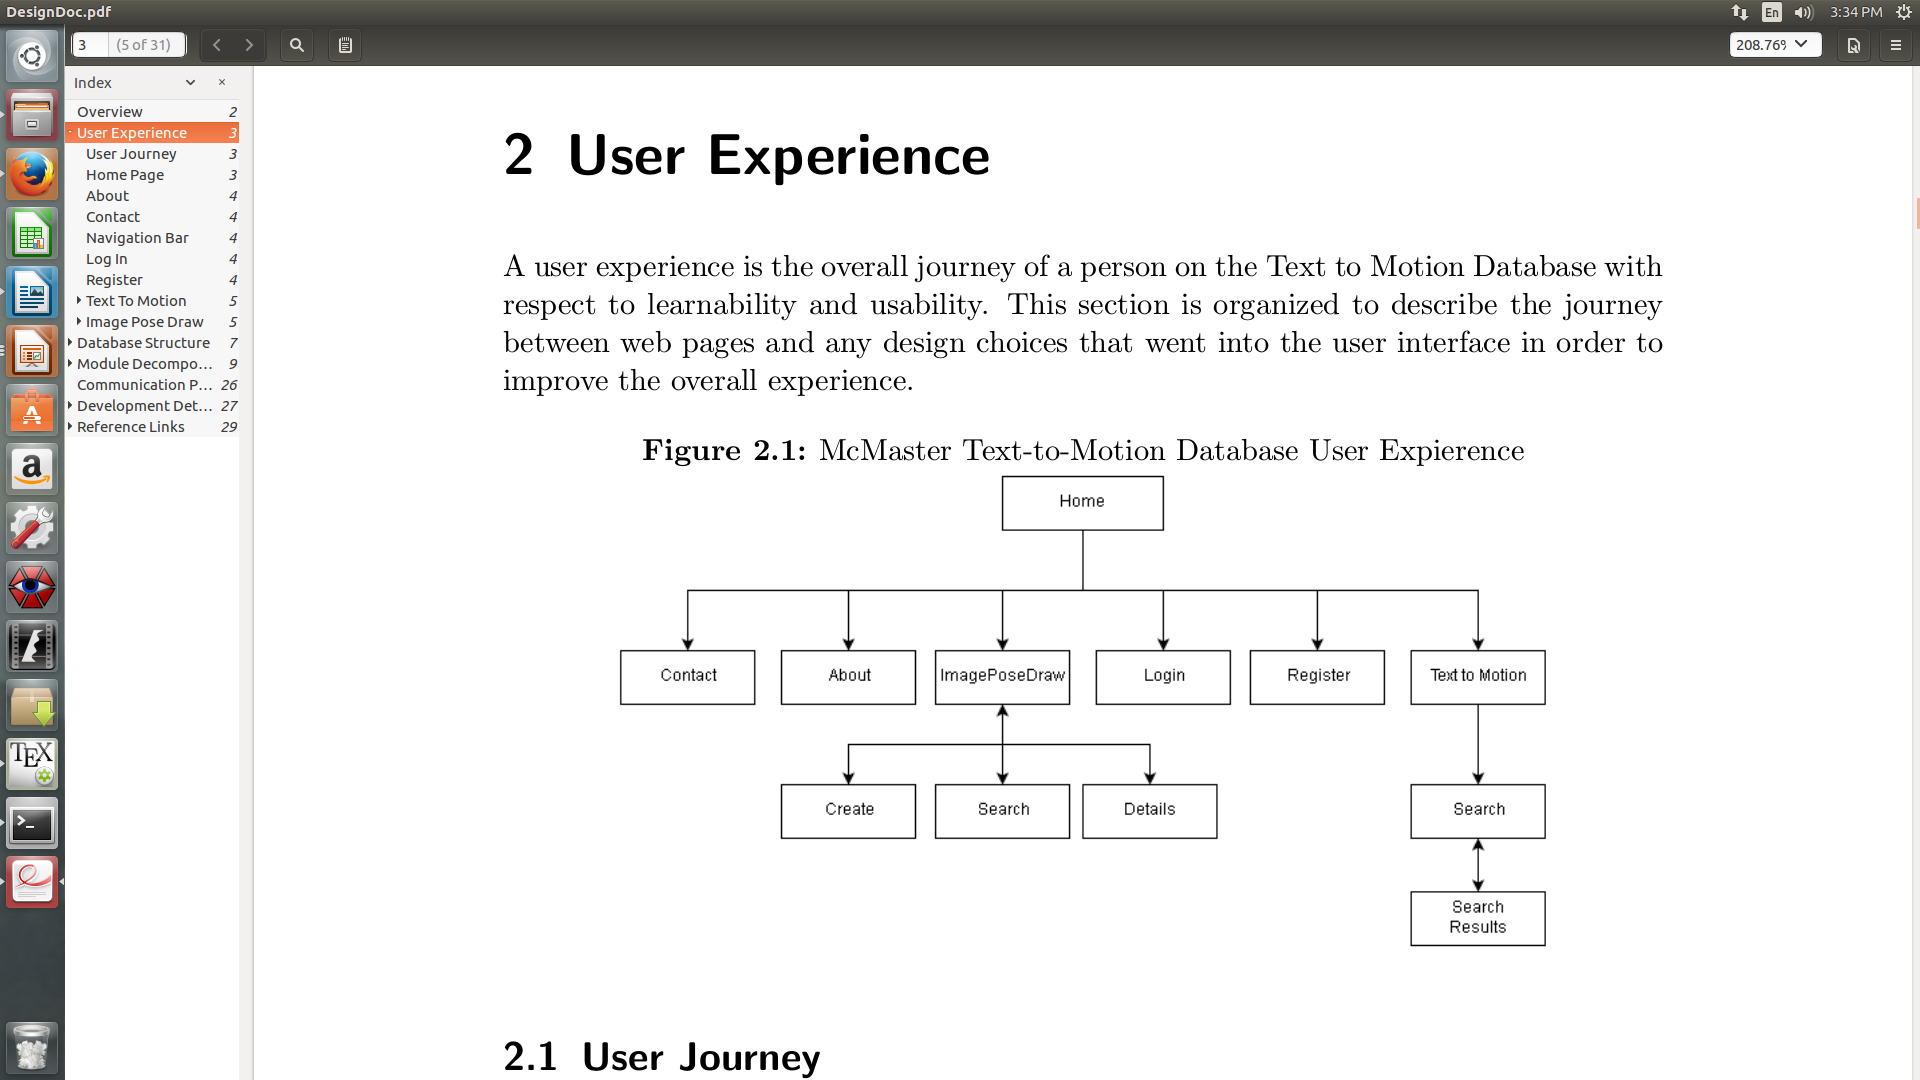
\includegraphics[width=\linewidth]{apppicture.png}
  \caption{Web Application Navigation Structure}
  \label{fig:navStruct}
\end{figure}

The navigational structure of our site is very simple.  If the navigation
starts at the Home page then any other page may be reached using a link from
this page.  The possible links are ImagePoseDraw, Login, Register, Contact and
About.

In Figure \ref{fig:navStruct} end point on this graph represents a
functionality that the application offers: create, search, details, contact,
about, login, register, search and search results.

The details, contact and about sections describe are actually pages that
display important data.  The contact page/function displays contact information
to get in contact with the creators of the software.  The about
page/functionality displays the information that describes motivation for the
web site.

For our site it is necessary to create a user profile to perform certain tasks.
The login and register functions allow users to create profiles and login to
their accounts.

Finally the search and search results allow users to search the data that is
stored by the web application and to display the results of their searches.

\subsubsection{Browser Requirements}

Currently our website is hosted at the address address 159.203.10.112:80. By
typing this address into a browser the Home page of our site should appear. The
specific page that should be seen in figure \ref{fig:homePage}

\begin{figure}
  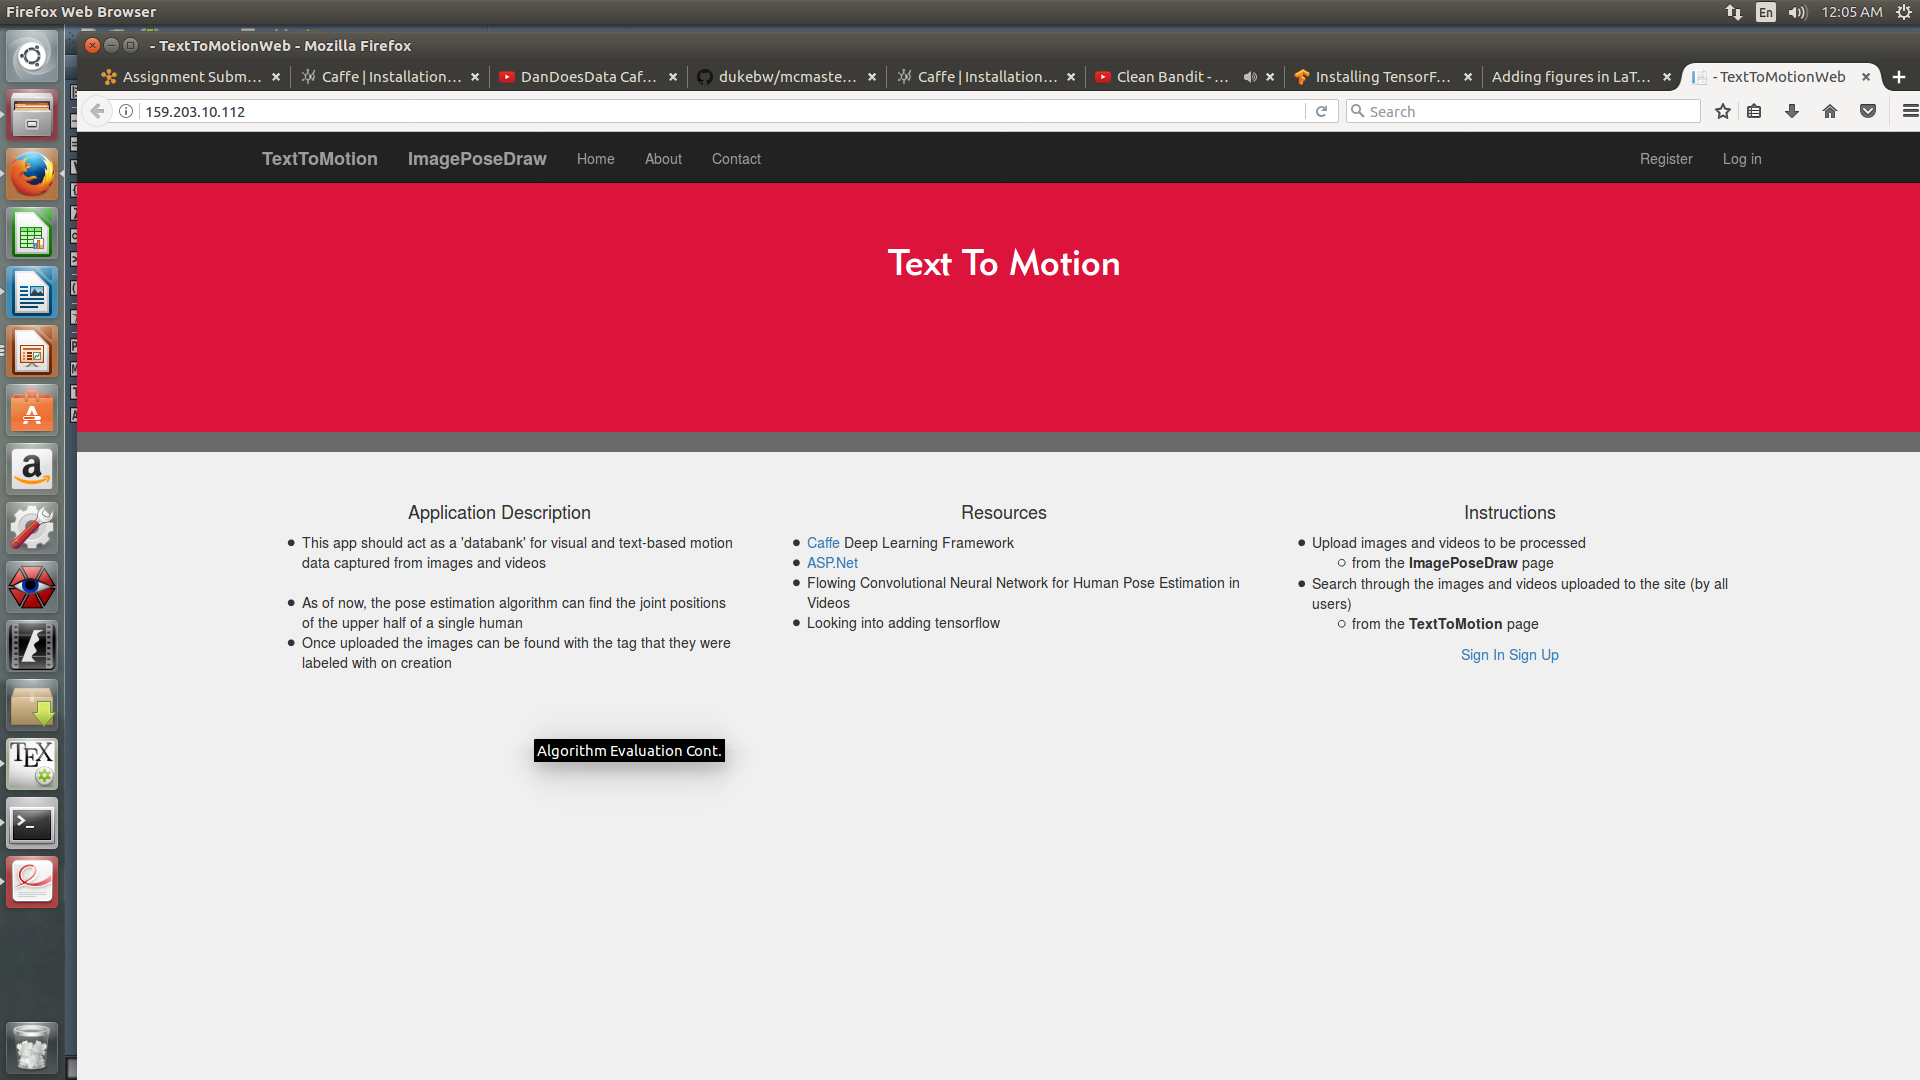
\includegraphics[width=\linewidth]{HomePage.png}
  \caption{Web Application Navigation Structure}
  \label{fig:homePage}
\end{figure}

This website can be accessed by any browser that supports HTML5.  Any
version of Internet Explorer more recent than version 6 should work and updated
verisons of Chrome and Firefox will work as well.

\subsubsection{Log In/Sign Up}

To use all of the features offered by the Text-To-Motion site users must create
a profile.  Without creating a profile data that is on the database may be
searched and displayed however to enter new data a user must have a profile and
be logged in.

\begin{figure}
  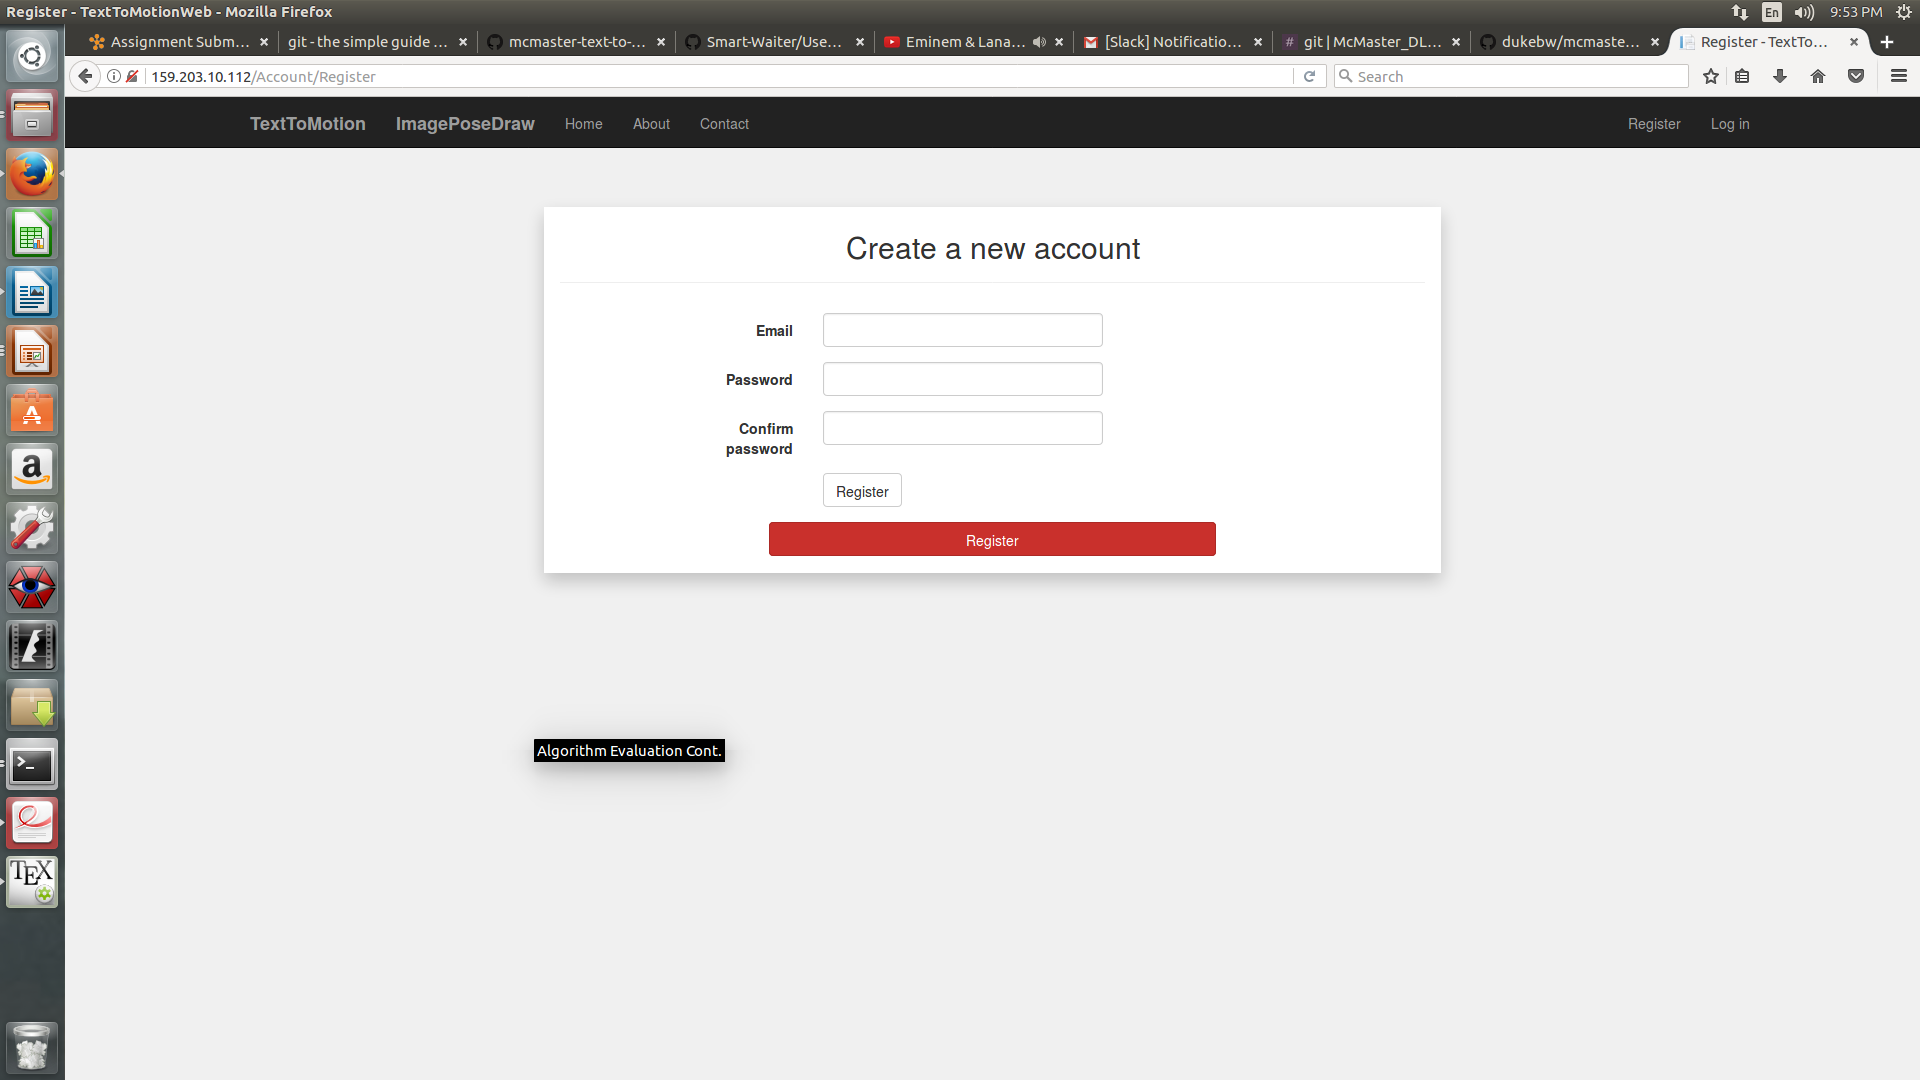
\includegraphics[width=\linewidth]{Register.png}
  \caption{Page Registration}
  \label{fig:regPage}
\end{figure}

To register as a user we can start at the home page and then click on the
register link.  Once this link has been clicked on the register page will
appear.  To register only an email address and password are necessary.

The password needs to be verified as can be seen in Figure \ref{fig:regPage}.
Once these fields are filled out and the register button is clicked a user
account will be created.  Note that each user account must have a unique email
address.

\subsubsection{Data Input}

The central feature of our application is in collecting and displaying data.
To navigate to the page that performs data input and displays already collected
data navigate to the home page and then click on the ImagePoseDraw link.

From this page data can be searched and inputted if the user is logged in.  To
input data simply click on the green button labelled "Add New Image" as shown
in Figure \ref{fig:uploadPage}.

\begin{figure}
  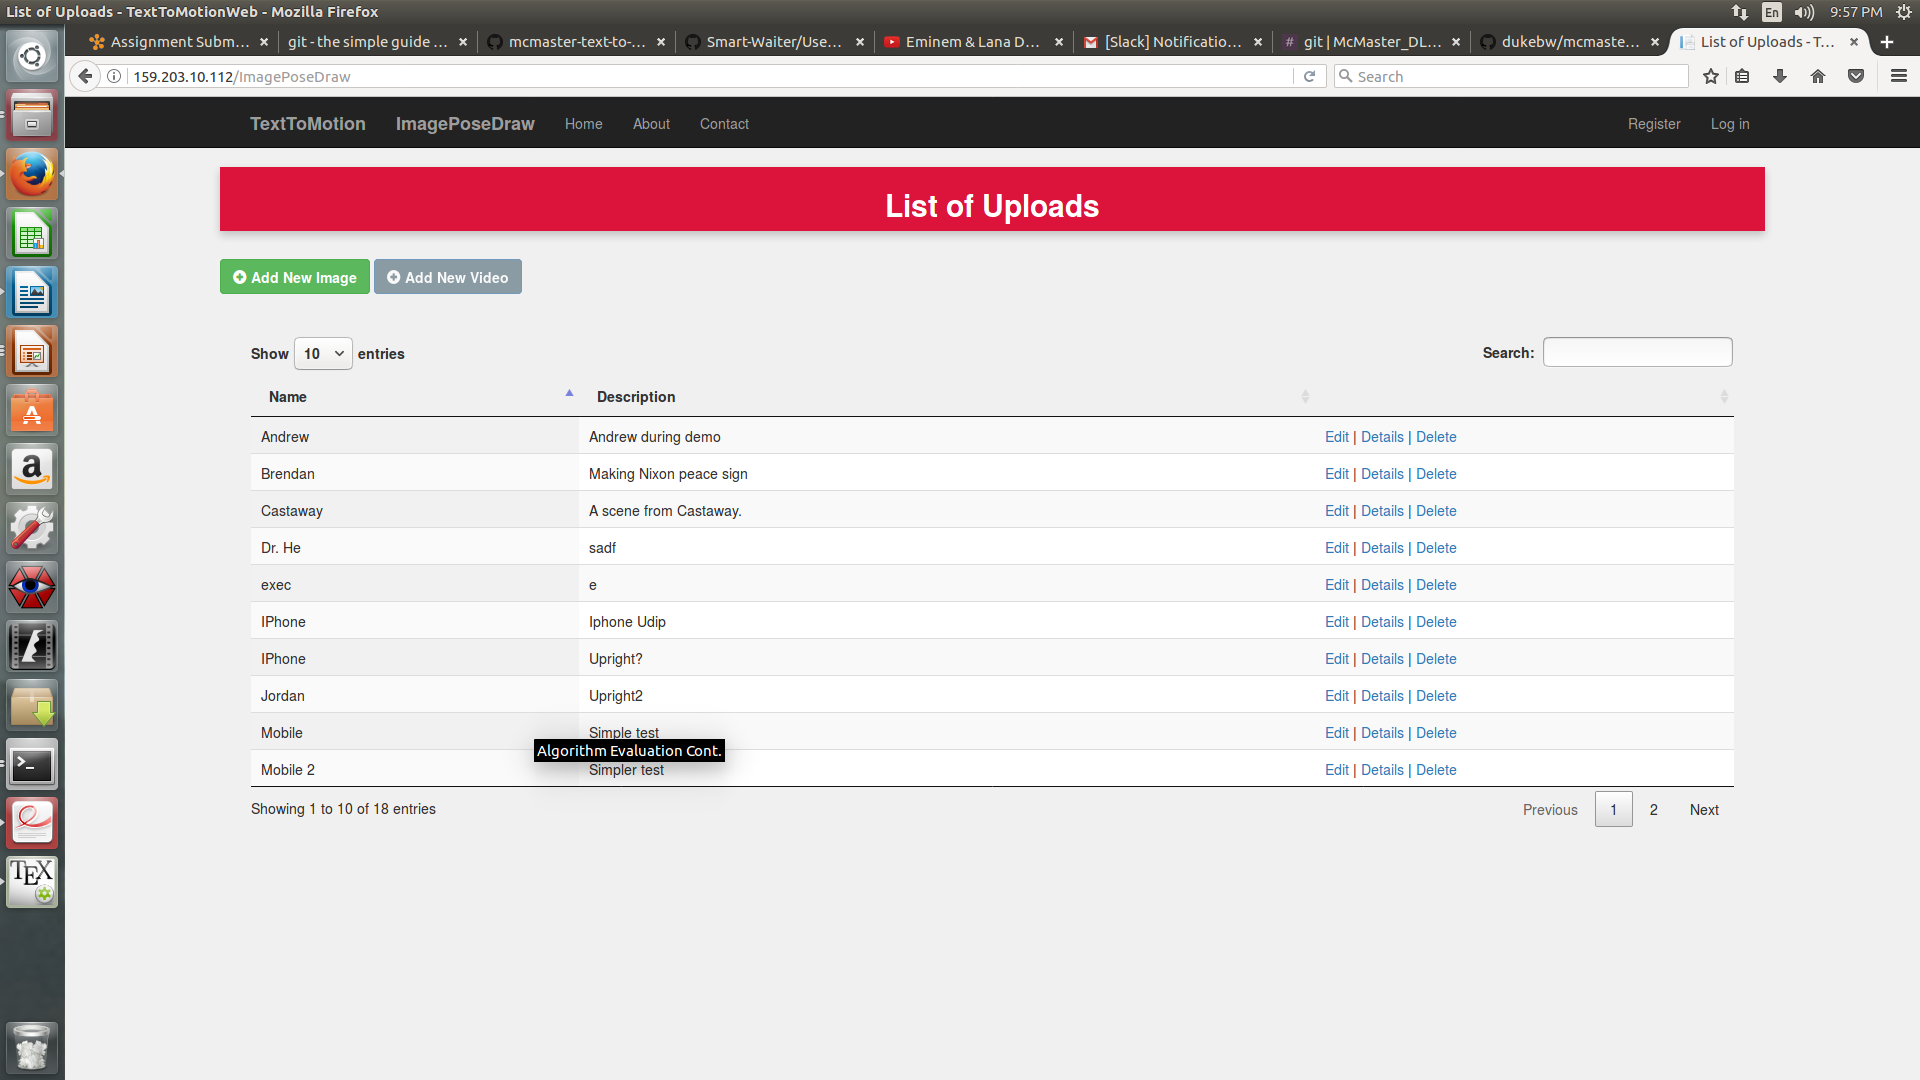
\includegraphics[width=\linewidth]{uploadPage.png}
  \caption{Uploading Image}
  \label{fig:uploadPage}
\end{figure}

After this button is clicked a new screen will appear that has 3 fields that
need to be filled out: filename, filepath and description.  The filepath is
entered by clicking on a new button that opens a user interface for a file
explorer which allows users to navigate the directories on their computer to
the location of the file they wish to upload.  Once the submit button is pushed
the appropriate file will be uploaded to our database and the file will be
labelled with the pixel locations that correspond to the joint positions.

\begin{figure}
  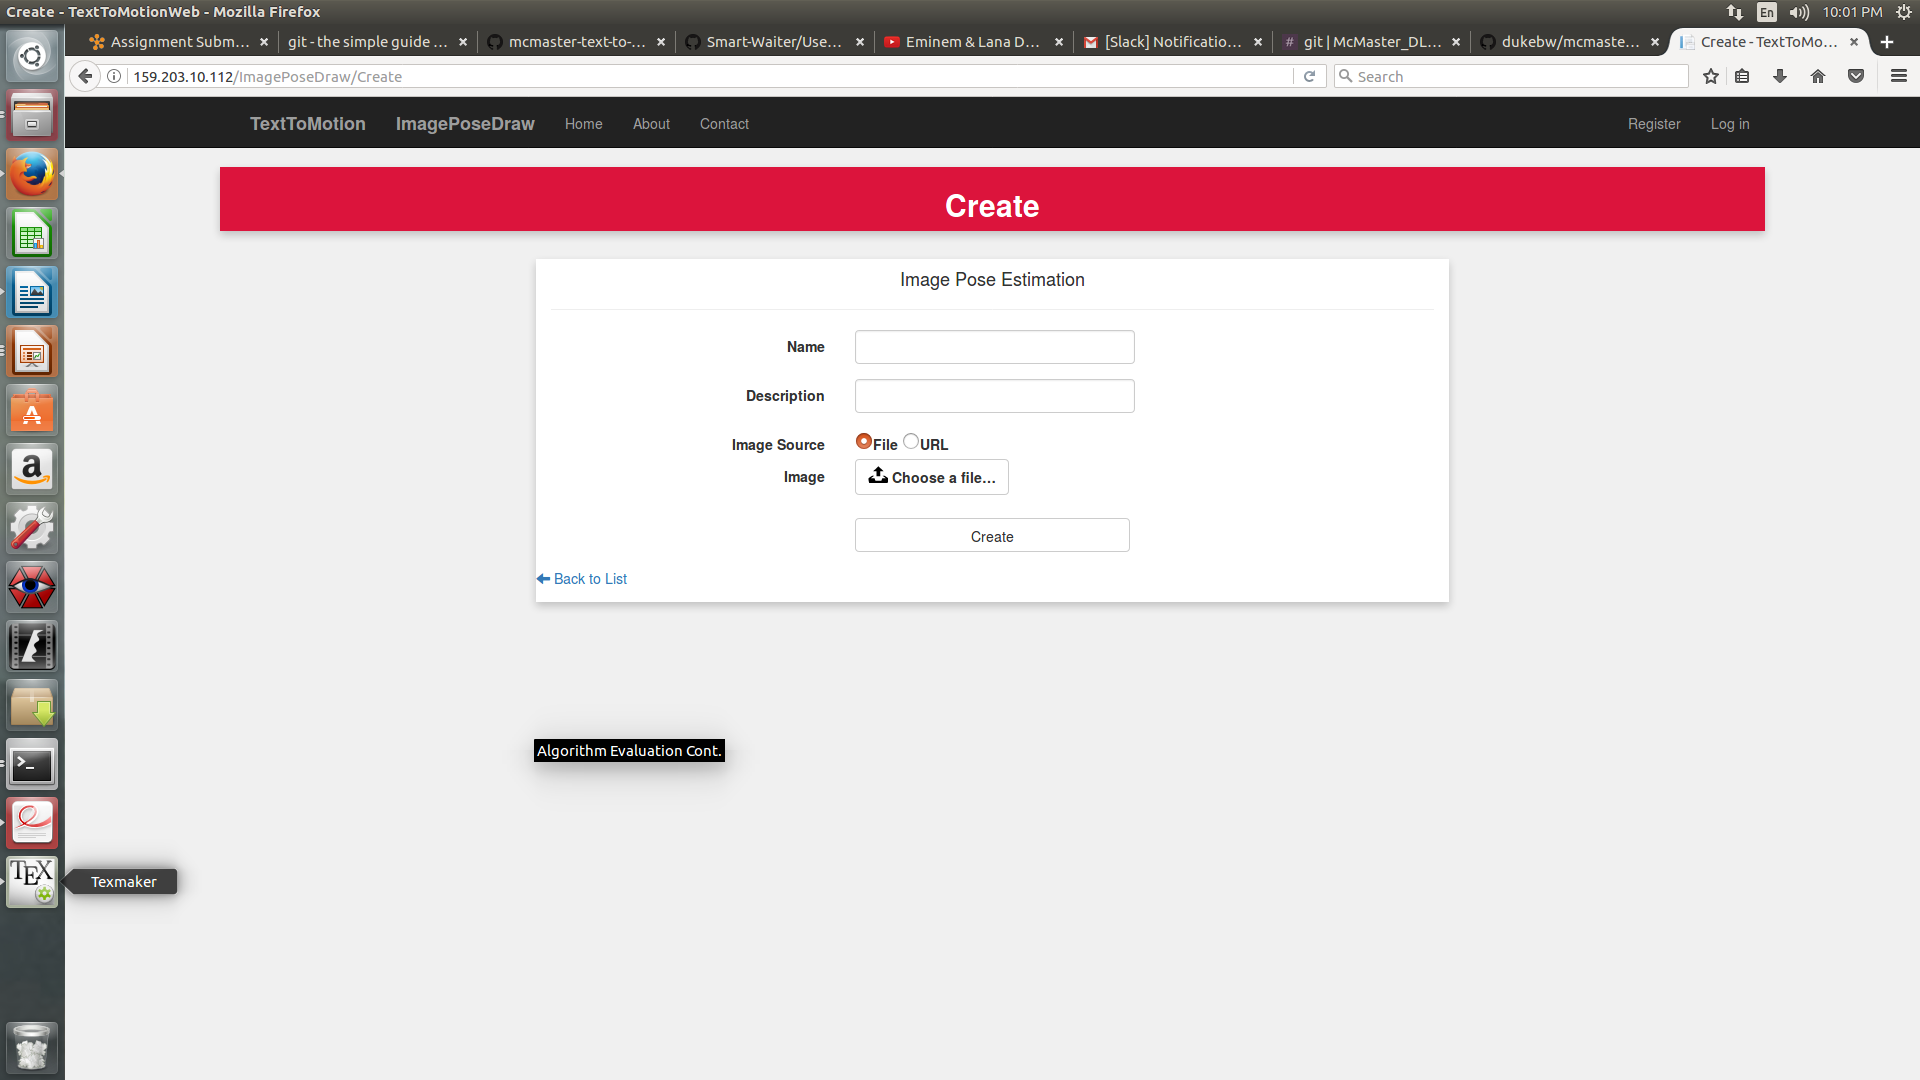
\includegraphics[width=\linewidth]{greenButtonPage.png}
  \caption{Entering Upload Data}
  \label{fig:uploadPage}
\end{figure}

Data restrictions are that the images file format must be in JPEG and PNG
formats.  Also the website is set up for downloading large data samples but a
limit of 2 minutes is set on the upload time.  Because of this the sample will
depend on the upload speed.

As an example of what the application can do we enter this image into the URL
shown in Figure \ref{fig:uploadPage}.

\begin{figure}
  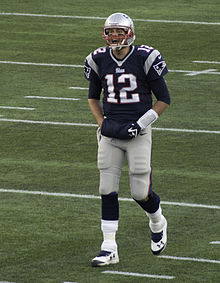
\includegraphics[width=\linewidth]{tbrady.jpg}
  \caption{Tom Brady}
  \label{fig:tomBrady}
\end{figure}

Then the results are obtained:

\begin{figure}
  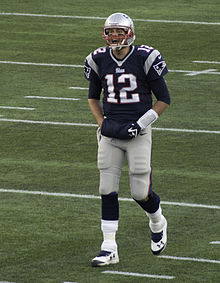
\includegraphics[width=\linewidth]{tbrady.jpg}
  \caption{Tom Brady Labelled}
  \label{fig:labelledBrady}
\end{figure}


\subsubsection{Data Search}

In addition to collecting and displaying data the application will allow users
to search through previous entries. From this page the user can search through
the database by inputting text on the bar that is located at the top of the
page. Once input, the entered text will be searched once the ``Enter'' key is hit
or the search button to the right is clicked. After the search has been
executed, the next page will display the results to the user with the text they
entered and the selected entries that match the description.

At this time the search function has not finished being implemented into the
application and will only display the text that was entered on the search page
as seen below.

% \begin{figure}
  % \includegraphics[width=\linewidth]{searchMan.jpg}
  % \caption{Search Page (Revision 0)}
  % \label{fig:searchPage}
% \end{figure}

\subsubsection{Troubleshooting}

Note that errors may result when images are uploaded.  The images must have a
JPEG or PNG format.  In addition large files that take more than 2 minutes to
upload will cause a timeout error.

For entering usernames and passwords we require that passwords have at least
one number, one letter, one capital and one non-alphanumeric character.
Uploading large files will only be allowed to take 2 minutes so that to upload
larger files will have to be broken up into smaller segments.


\subsection{Errors or overwriting Data}

For users each user must create a unique username.  If a user uses a username
that is already in use a error message will be shown to the user and they will
be asked to enter a new name.  Multiple users can share the same password
however.

For entering and videos no limit or restrictions are set for duplications.  So
the same image or video may be uploaded many times without causing overwriting
to occur.  However if the user wishes to avoid duplication they can search the
database for specific pictures or videos using the search function.


\section{Roadmap: Service Providers}

As previously mentioned the software is for a  web application which runs a
computationally expensive image/video analysis on its backend. To store the
large amounts of data a database server is needed for hosting.  In addition we
wish to query the database so a search library is also needed. Then to perform
the calculation a machine learning library is used and finally to host a web
framework is needed. All of these components need to be installed separately.

The specific software tools, packages and libraries that need to be available
to the system to run our software are:

\begin{itemize}
  \item Python version 3.x
  \item ASP.Net MVC
  \item MySQL
  \item Caffe
  \item TensorFlow
  \item Sphinx search library
\end{itemize}



\subsection{Installation}

The software project we have developed is available on GitHub:
https://github.com/dukebw/mcmaster-text-to-motion-database and can be
downloaded by cloning our repository.

Instructions on using GitHub are available at this address:

However if the user is running a Linux system the repository can be downloaded
by typing in the clone command from the terminal screen:

\begin{lstlisting}

git clone --recursive https://github.com/dukebw/
mcmaster-text-to-motion-database

\end{lstlisting}

However the software we have developed has several dependencies which fall
under the three categories we have decomposed the project into: database,
machine learning libraries, and the web framework.  Python is a central
language used in our project is in nearly all of these modules.  We assume
python version 3.5 or higher is installed.


\subsection{System Requirements}

\begin{itemize}
\item GHz or faster processor
\item 512 MB of RAM
\item Ubuntu 16.04 with basic configuration (e.g. port 80 opened, packages updated)
\end{itemize}


\subsection{Troubleshooting}

\section{Frequently asked Questions}

Question 1: How can I improve the fit given by the program?

Answer 1 : One improvement would be to try and use pictures that have only a single person in them.

Question 2: How can I upload large files?

Answer 2: We are currently working on a web feature for large uploads.

Question 3: What algorithms are used by the program?

Answer 3: The algorithms that were used are outlined in [1].

Question 4:

Answer 4:

\begin{thebibliography}{9}

\bibitem{latexcompanion}
Bulat, Adrian, Tzimiropoulos, Georgios.
\textit{Human pose estimation via Convulutional Part Heatmap Regression}.
eprint arXiv: 1609.01743.

\end{thebibliography}

\end{document}
